\section{Evaluation}\label{sec:eval}

We evaluate \sysname{} using a combination of testbed experiments and numerical experiments. Our evaluation centers around four key questions:

\begin{itemize}
	\item \textbf{Can \sysname{} prevent deadlock when deadlock-prone misconfiguration or network failure happens?}
	
	\item \textbf{Is \sysname{} scalable for large scale datacenters?}
	
	\item \textbf{Can \sysname{} work at full line rate with little performance overhead?}
	
	\item \textbf{Does the mechanism of priority reusing cause any inefficiency or unfairness problem?} 
	
\end{itemize}


\subsection{Lossless transition between priority classes}\label{subsec:exp_losslesstransition}

%\begin{figure}[t]
%	%\vspace{-0.1in}
%	\centering
%	
%	\subfloat[short for lof][] {
%		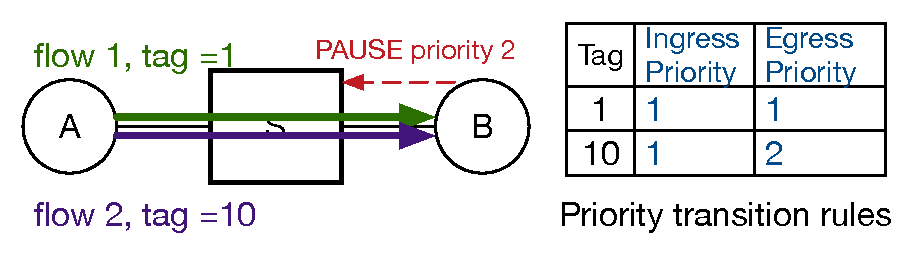
\includegraphics[width=0.43\textwidth] {figs/exp_queuetransition_1}
%	}
%	
%	\vspace{-0.15in}
%	\subfloat[short for lof][]{
%		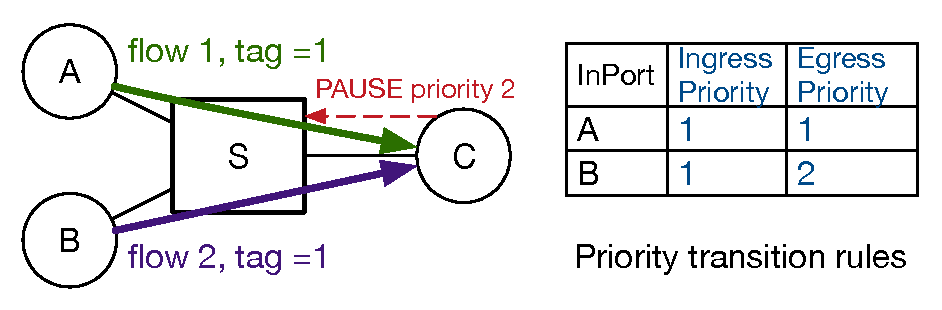
\includegraphics[width=0.43\textwidth] {figs/exp_queuetransition_2}
%	}
%
%\vspace{-0.15in}
%	\subfloat[short for lof][]{
%	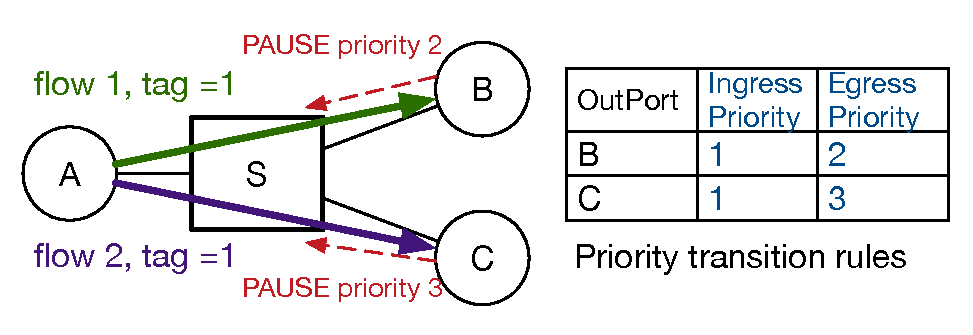
\includegraphics[width=0.43\textwidth] {figs/exp_queuetransition_3}
%     }
%	
%	\caption{Experiment scenarios to demonstrate lossless transition between priority classes.}\label{fig:exp_queuetransition}
%\end{figure}

\textbf{Purpose:} demonstrate our implementation ensures lossless transition between priority classes.

\textbf{Scenario-1:} As shown in Fig.~\ref{fig:exp_queuetransition}(a), by pausing priority 2 at server B, flow 2 is paused correctly without any packet loss, while flow 1 is not affected.

\textbf{Scenario-2:} As shown in Fig.~\ref{fig:exp_queuetransition}(b), by pausing priority 2 at server C, flow 2 is paused correctly without any packet loss, while flow 1 is not affected.

\textbf{Scenario-3:} The scenario is shown in Fig.~\ref{fig:exp_queuetransition}(c). By pausing priority 2 at server B, flow 1 is paused correctly without any packet loss. By pausing priority 3 at server C, flow 2 is paused correctly without any packet loss.

\subsection{Validation}\label{subsec:exp_validation}

\begin{figure}[t]
	%\vspace{-0.1in}
	\centering
	
	\subfloat[short for lof][] {
		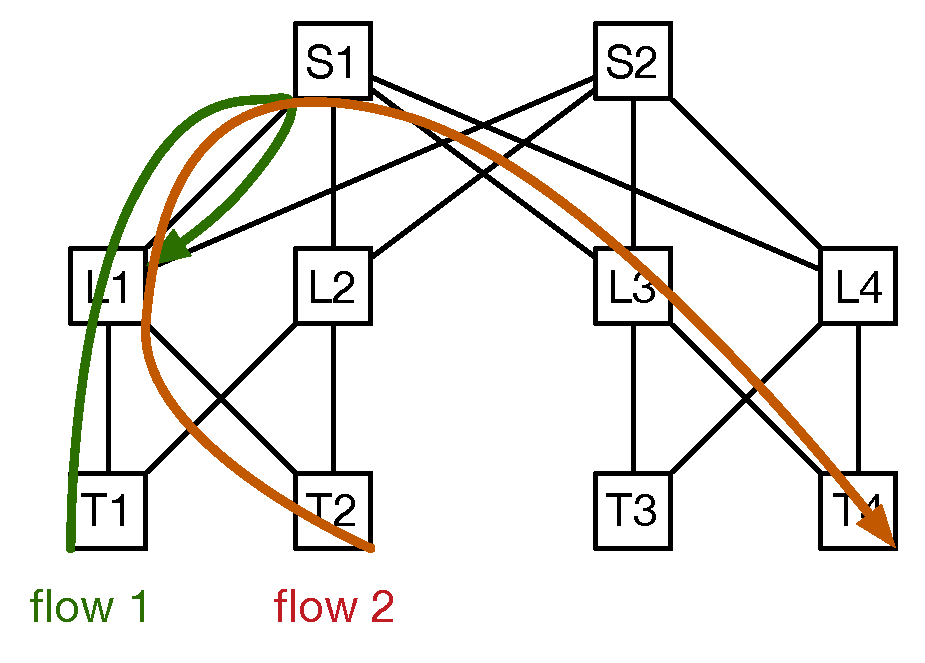
\includegraphics[width=0.25\textwidth] {figs/validation_1}
	}
	\subfloat[short for lof][]{
		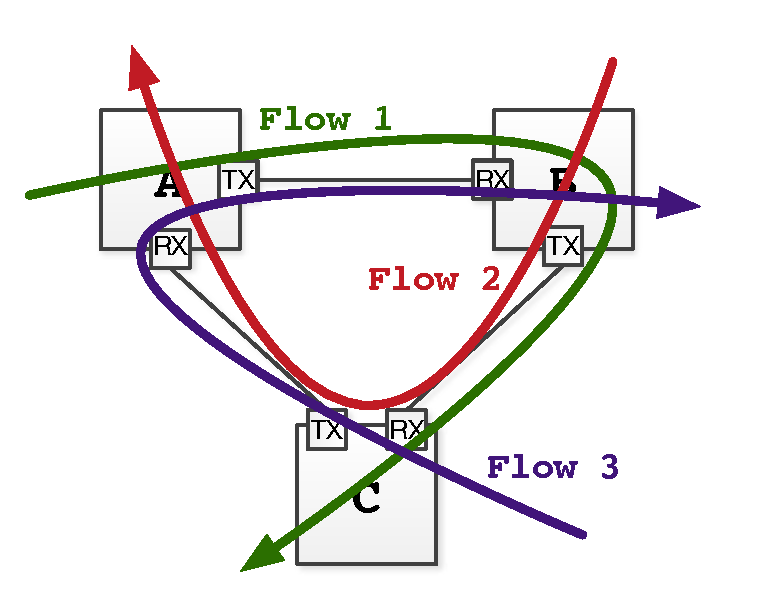
\includegraphics[width=0.25\textwidth] {figs/validation_2}
	}
	
	\caption{Scenarios of validation experiment.}\label{fig:exp_validation}
	
\end{figure}

\textbf{Purpose:} demonstrate our solution can prevent deadlock.

\textbf{Scenario-1:} As shown in Fig.~\ref{fig:exp_validation}(a), In a Clos network, we generate 2 flows across different ToRs. Flow 1 enters a routing loop due to misconfiguration, and forms a deadlock. Without \sysname{}, flow 2 will also get paused due to propagation of PFC PAUSE. With \sysname{}, there is no deadlock and flow 2 is not affected by the routing loop.

\textbf{Scenario-2:} As shown in Fig.~\ref{fig:exp_validation}(b), we inject 3 flows into three paths that contain a CBD. Without \sysname{}, deadlock occurs and three flows are all paused. With \sysname{}, there is no deadlock and three flows achieve good throughput.

\subsection{Overhead}\label{subsec:exp_overhead}

\subsubsection{Resource Consumption}\label{subsec:exp_resourceconsump}

\textbf{Purpose:} demonstrate our solution only consumes a small number of priorities and ACL entries.

\textbf{Scenario:} for Fattree, BCube and Jellyfish, we calculate the following metrics under different network scales to show \sysname{} is scalable in terms of resource consumption.
\begin{enumerate}
	\item $\#$ of lossless priorities;
	\item $\#$ of total ACL rules;
 	\item $\#$ of ACL rules at the bottleneck switch.
\end{enumerate}

\subsubsection{Performance overhead}\label{subsec:exp_performanceoverhead}

 \textbf{Purpose:} demonstrate performance overhead of \sysname{} is small.

\textbf{Scenario-1:} We let a flow traverse $m$ hops in the network, and perform tagging and priority manipulation at every hop. We can evaluate the performance overhead of \sysname{} by measuring the throughput and latency when using different values of $m$.

\textbf{Scenario-2:} we increase the $\#$ of ACL rules installed in a switch, and observe the performance overhead of the flows passing over this switch.

\subsection{Impact of priority reusing}\label{subsec:exp_priorityreusing}


\begin{figure}
	%\vspace{-0.1in}
	\centering
	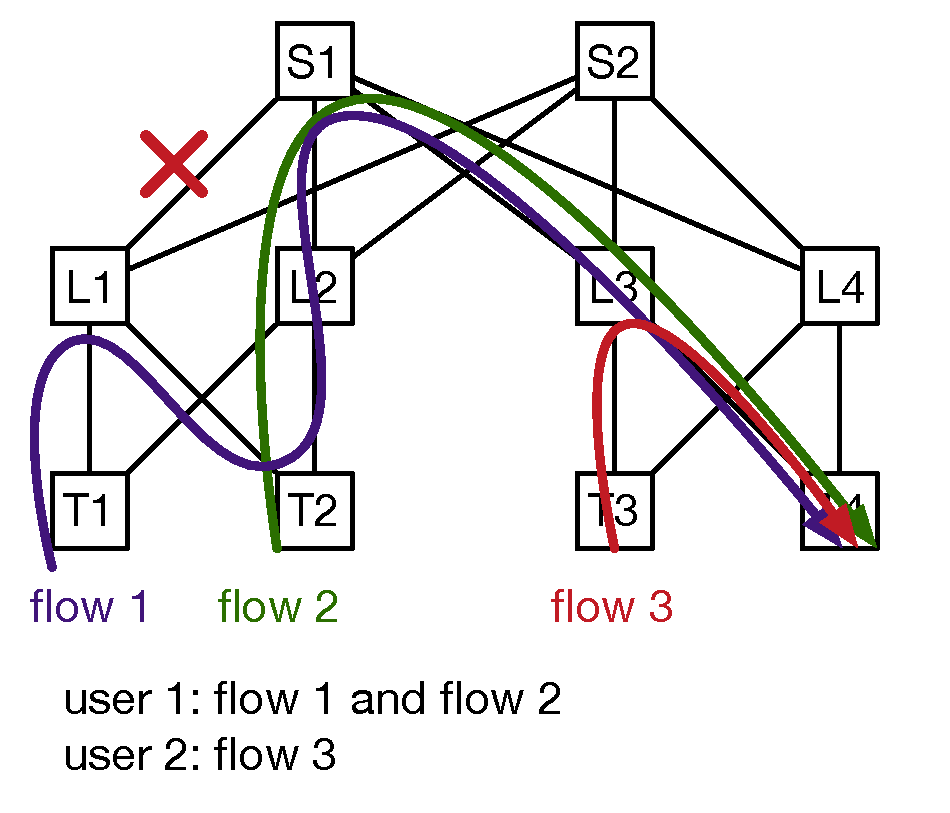
\includegraphics[width=0.45\textwidth] {figs/priorityreusing_1}
	\caption{Scenario of priority reusing experiment.}\label{fig:exp_priorityreusing}
	
\end{figure}

\textbf{Purpose:} demonstrate the mechanism of priority reusing will not downgrade link utilization and throughput of flows (but may introduce unfairness problem).

\textbf{Scenario:} As shown in Fig.~\ref{fig:exp_priorityreusing}(a), a Clos network serves two users belonging to different application classes. For user 1, priority 1 is used for traffic following shortest paths, and priority 2 is used for traffic following 1-bounce paths. For user 2, priority 2 is used for traffic following shortest paths, and priority 1 is used for traffic following 1-bounce paths.

Assuming WRR policy among different egress queues. Assuming traffic of these two users shares a bottleneck link. We create a link failure to let flow 1 of user 1 enter the second lossless space. Flow 1 then competes link bandwidth in the same egress queue with flow 3 of user 2 at the bottleneck link L3-T4. 

By measuring the link utilization and throughput of all flows, we can demonstrate that link utilization of the bottleneck link and overall throughput of all flows is not downgraded, but priority reusing does cause some unfairness problem among different suers.

\textbf{compared scheme:} no priority reusing among users (4 priorities are used)
  
\subsection{Hierarchical lossless space improves application performance}\label{subsec:exp_appperformance}

\textcolor{red}{This experiment will be moved to Section 3 as an motivation experiment.}

\textbf{Purpose:} demonstrate that for Clos network, applications can achieve better performance when both shortest paths and 1 bounce paths are lossless.

\textbf{Scenario:} In a Clos network, we run both throughput-intensive and latency-sensitive applications. We randomly generate k failures in the network to have some of the flows follow 1-bounce paths.

 \textbf{compared schemes:}
 \begin{enumerate}
 	\item both shortest paths and  1 bounce paths are lossless.
 	\item shortest paths are lossless. 1 bounce paths are lossy.
 	\item Only shortest paths are allowed.
 \end{enumerate}
  
%   \subsection{Experiment 7: dealcok-free reconfiguration of ACL rules.}\label{subsec:exp_acloverhead}
%   
%   \textbf{Point to demonstrate:} when operator changes the topology or desired routing, we can do an online dealcok-free reconfiguration of ACL rules.
%   
%    \textcolor{red}{need a solution to do dealcok-free reconfiguration of ACL rules at first.}
    
    
    % \subsection{Experiment 2: CBD probability}\label{subsec:exp_CBDprobability}
    % 
    % \textbf{Point to demonstrate:} it is easy for a network to have CBD.
    % 
    % \textbf{Setup:} for Fattree, we randomly generate k failures or misconfiguration, and evaluate whether CBD is created.
    % 
    %  for BCube and Jellyfish, we calculate the default lossless routing by randomly choosing m shortest paths between each node pair. And then we check whether the output routing includes CBD.
  